\documentclass[twoside]{article}

%%%%%%%%%%%%%%%%%%%%%%%%%%%%%%%%%%%%%%%%%
% Lachaise Assignment
% Structure Specification File
% Version 1.0 (26/6/2018)
%
% This template originates from:
% http://www.LaTeXTemplates.com
%
% Authors:
% Marion Lachaise & François Févotte
% Vel (vel@LaTeXTemplates.com)
%
% License:
% CC BY-NC-SA 3.0 (http://creativecommons.org/licenses/by-nc-sa/3.0/)
%
%%%%%%%%%%%%%%%%%%%%%%%%%%%%%%%%%%%%%%%%%

%----------------------------------------------------------------------------------------
%	PACKAGES AND OTHER DOCUMENT CONFIGURATIONS
%----------------------------------------------------------------------------------------

\usepackage{amsmath,amsfonts,stmaryrd,amssymb} % Math packages

\usepackage{enumerate} % Custom item numbers for enumerations

% \usepackage[ruled]{algorithm2e} % Algorithms

\usepackage[framemethod=tikz]{mdframed} % Allows defining custom boxed/framed environments

\usepackage{listings} % File listings, with syntax highlighting
\lstset{
	basicstyle=\ttfamily, % Typeset listings in monospace font
}

\usepackage[hmarginratio=1:1,top=32mm,columnsep=20pt]{geometry} % Document margins

%----------------------------------------------------------------------------------------
%	DOCUMENT MARGINS
%----------------------------------------------------------------------------------------

% \usepackage{geometry} % Required for adjusting page dimensions and margins

\geometry{
	paper=a4paper, % Paper size, change to letterpaper for US letter size
	top=2.5cm, % Top margin
	bottom=3cm, % Bottom margin
	left=2.5cm, % Left margin
	right=2.5cm, % Right margin
	headheight=14pt, % Header height
	footskip=1.5cm, % Space from the bottom margin to the baseline of the footer
	headsep=1.2cm, % Space from the top margin to the baseline of the header
	%showframe, % Uncomment to show how the type block is set on the page
}

%----------------------------------------------------------------------------------------
%	FONTS
%----------------------------------------------------------------------------------------

\usepackage[utf8]{inputenc} % Required for inputting international characters
\usepackage[T1]{fontenc} % Output font encoding for international characters

\usepackage{XCharter} % Use the XCharter fonts

%----------------------------------------------------------------------------------------
%	COMMAND LINE ENVIRONMENT
%----------------------------------------------------------------------------------------

% Usage:
% \begin{commandline}
%	\begin{verbatim}
%		$ ls
%
%		Applications	Desktop	...
%	\end{verbatim}
% \end{commandline}

\mdfdefinestyle{commandline}{
	leftmargin=10pt,
	rightmargin=10pt,
	innerleftmargin=15pt,
	middlelinecolor=black!50!white,
	middlelinewidth=2pt,
	frametitlerule=false,
	backgroundcolor=black!5!white,
	frametitle={Command Line},
	frametitlefont={\normalfont\sffamily\color{white}\hspace{-1em}},
	frametitlebackgroundcolor=black!50!white,
	nobreak,
}

% Define a custom environment for command-line snapshots
\newenvironment{commandline}{
	\medskip
	\begin{mdframed}[style=commandline]
}{
	\end{mdframed}
	\medskip
}

%----------------------------------------------------------------------------------------
%	FILE CONTENTS ENVIRONMENT
%----------------------------------------------------------------------------------------

% Usage:
% \begin{file}[optional filename, defaults to "File"]
%	File contents, for example, with a listings environment
% \end{file}

\mdfdefinestyle{file}{
	innertopmargin=1.6\baselineskip,
	innerbottommargin=0.8\baselineskip,
	topline=false, bottomline=false,
	leftline=false, rightline=false,
	leftmargin=2cm,
	rightmargin=2cm,
	singleextra={%
		\draw[fill=black!10!white](P)++(0,-1.2em)rectangle(P-|O);
		\node[anchor=north west]
		at(P-|O){\ttfamily\mdfilename};
		%
		\def\l{3em}
		\draw(O-|P)++(-\l,0)--++(\l,\l)--(P)--(P-|O)--(O)--cycle;
		\draw(O-|P)++(-\l,0)--++(0,\l)--++(\l,0);
	},
	nobreak,
}

% Define a custom environment for file contents
\newenvironment{file}[1][File]{ % Set the default filename to "File"
	\medskip
	\newcommand{\mdfilename}{#1}
	\begin{mdframed}[style=file]
}{
	\end{mdframed}
	\medskip
}

%----------------------------------------------------------------------------------------
%	NUMBERED QUESTIONS ENVIRONMENT
%----------------------------------------------------------------------------------------

% Usage:
% \begin{question}[optional title]
%	Question contents
% \end{question}

\mdfdefinestyle{question}{
	innertopmargin=1.2\baselineskip,
	innerbottommargin=0.8\baselineskip,
	roundcorner=5pt,
	nobreak,
	singleextra={%
		\draw(P-|O)node[xshift=1em,anchor=west,fill=white,draw,rounded corners=5pt]{%
		Question \theQuestion\questionTitle};
	},
}

\newcounter{Question} % Stores the current question number that gets iterated with each new question

% Define a custom environment for numbered questions
\newenvironment{question}[1][\unskip]{
	\bigskip
	\stepcounter{Question}
	\newcommand{\questionTitle}{~#1}
	\begin{mdframed}[style=question]
}{
	\end{mdframed}
	\medskip
}

%----------------------------------------------------------------------------------------
%	WARNING TEXT ENVIRONMENT
%----------------------------------------------------------------------------------------

% Usage:
% \begin{warn}[optional title, defaults to "Warning:"]
%	Contents
% \end{warn}

\mdfdefinestyle{warning}{
	topline=false, bottomline=false,
	leftline=false, rightline=false,
	nobreak,
	singleextra={%
		\draw(P-|O)++(-0.5em,0)node(tmp1){};
		\draw(P-|O)++(0.5em,0)node(tmp2){};
		\fill[black,rotate around={45:(P-|O)}](tmp1)rectangle(tmp2);
		\node at(P-|O){\color{white}\scriptsize\bf !};
		\draw[very thick](P-|O)++(0,-1em)--(O);%--(O-|P);
	}
}

% Define a custom environment for warning text
\newenvironment{warn}[1][Warning:]{ % Set the default warning to "Warning:"
	\medskip
	\begin{mdframed}[style=warning]
		\noindent{\textbf{#1}}
}{
	\end{mdframed}
}

%----------------------------------------------------------------------------------------
%	INFORMATION ENVIRONMENT
%----------------------------------------------------------------------------------------

% Usage:
% \begin{info}[optional title, defaults to "Info:"]
% 	contents
% 	\end{info}

\mdfdefinestyle{info}{%
	topline=false, bottomline=false,
	leftline=false, rightline=false,
	nobreak,
	singleextra={%
		\fill[black](P-|O)circle[radius=0.4em];
		\node at(P-|O){\color{white}\scriptsize\bf i};
		\draw[very thick](P-|O)++(0,-0.8em)--(O);%--(O-|P);
	}
}

% Define a custom environment for information
\newenvironment{info}[1][Info:]{ % Set the default title to "Info:"
	\medskip
	\begin{mdframed}[style=info]
		\noindent{\textbf{#1}}
}{
	\end{mdframed}
}
 % Include the file specifying the document structure and custom commands

\usepackage[sc]{mathpazo} % Use the Palatino font
\usepackage[T1]{fontenc} % Use 8-bit encoding that has 256 glyphs
\linespread{1.05} % Line spacing - Palatino needs more space between lines
\usepackage{microtype} % Slightly tweak font spacing for aesthetics

% \usepackage[noadjust]{cite}

\usepackage[english]{babel} % Language hyphenation and typographical rules

% \usepackage[hmarginratio=1:1,top=32mm,columnsep=20pt]{geometry} % Document margins
\usepackage[hang, small,labelfont=bf,up,textfont=it,up]{caption} % Custom captions under/above floats in tables or figures
\usepackage{booktabs} % Horizontal rules in tables

\usepackage{lettrine} % The lettrine is the first enlarged letter at the beginning of the text

\usepackage{enumitem} % Customized lists
\setlist[itemize]{noitemsep} % Make itemize lists more compact

\usepackage{abstract} % Allows abstract customization
\renewcommand{\abstractnamefont}{\normalfont\bfseries} % Set the "Abstract" text to bold
\renewcommand{\abstracttextfont}{\normalfont\small\itshape} % Set the abstract itself to small italic text

\usepackage{titlesec} % Allows customization of titles
\renewcommand\thesection{\Roman{section}} % Roman numerals for the sections
\renewcommand\thesubsection{\roman{subsection}} % roman numerals for subsections
\titleformat{\section}[block]{\large\scshape}{\thesection.}{1em}{} % Change the look of the section titles
\titleformat{\subsection}[block]{\large}{\thesubsection.}{1em}{} % Change the look of the section titles

\usepackage{fancyhdr} % Headers and footers
\pagestyle{fancy} % All pages have headers and footers
\fancyhead{} % Blank out the default header
\fancyfoot{} % Blank out the default footer
\fancyhead[C]{Parallel GPU Implementation of the 2D Lattice-Boltzmann Method in Julia $\bullet$ May 2020} % Custom header text
\fancyfoot[RO,LE]{\thepage} % Custom footer text

\usepackage{titling} % Customizing the title section
\usepackage{hyperref} % For hyperlinks in the PDF
\usepackage{graphicx}
\usepackage{amsmath}
\usepackage{bm}
\usepackage{tocbibind}
\usepackage[toc, page]{appendix}
\usepackage{subcaption}
\usepackage{multirow}
\usepackage{float}
\usepackage{algorithm}
\usepackage{algorithmic}


\renewcommand{\appendixpagename}{Appendix}

% Simple function to create multiline comment
\newcommand{\comment}[1]{}


%----------------------------------------------------------------------------------------
%	TITLE SECTION
%----------------------------------------------------------------------------------------

\setlength{\droptitle}{-4\baselineskip} % Move the title up

\pretitle{\begin{center}\Huge\bfseries} % Article title formatting
\posttitle{\end{center}} % Article title closing formatting
\title{Parallel GPU Implementation of the 2D Lattice-Boltzmann Method in Julia} % Article title
\author{%
\textsc{Ryan French} \\[1ex] % Your name
\normalsize Montana State University \\ % Your institution
\normalsize ryanfrenchphysics@gmail.com % Your email address
}

\date{\today} % Leave empty to omit a date
\renewcommand{\maketitlehookd}{%
\begin{abstract}
An efficient approach for modeling two-dimensional, nonturbulent fluid dynamics is proposed that combines the speed of GPU-parallelized code and the power of Julia's JIT compiler. The model is derived from the Lattice-Boltzmann Method and is tightly-coupled to Julia's compact user-defined types and multiple dispatch paradigm. The Julia library executing this model, while limited, is easily extensible to models that are more demanding.
\end{abstract}
}

%----------------------------------------------------------------------------------------

\begin{document}
\setlength{\abovedisplayskip}{6pt}
\setlength{\belowdisplayskip}{6pt}

% Print the title
\maketitle

%----------------------------------------------------------------------------------------
%	ARTICLE CONTENTS
%----------------------------------------------------------------------------------------

\section{Introduction}
\subsection*{Lattice-Boltzmann Method}

Macroscopic computational fluid dynamics (CFD) is dominated by iterative forms of the Navier-Stokes equations, which is derived from applying classical conservation laws to fluids, along with terms describing viscosity and pressure. Methods derived from Navier-Stokes are very accurate and provide the best macroscopic solutions to a variety of problems in physics and engineering. \\

\noindent Bridging the gap between macroscopic and microscopic CFD methods is the Lattice-Boltzmann method (LBM), a relatively recent development forged from the method of Lattice gas automata (LGA). LGA, which is based on a d-dimensional lattice, suffered from non-Galilean invariance and unphysical pressure and viscosity relationships. In 1988, McNamara and Zanetti\cite{McNamaraZanetti} modified LGA by neglecting particle correlations and introducing averaged distribution functions. Later, Higuera and Jimenez\cite{HigueraJimenez} presented a Lattice Boltzmann Equation, which featured a linearized collision operator that assumes a local near-equilibrium state\cite{PerumalDass:2015Review}.\\

\noindent Because LBM is a mesoscopic theory based around distribution functions within a small volume element, the results from this theory are easily transformed into macroscopic results (in fact, it is possible to derive the Navier-Stokes equations from Lattice-Boltzmann equations). See\cite{ChenDoolen} for the full derivation. This fact presents LBM as a viable method of CFD, as opposed to current finite-difference and finite-volume methods.\\

\noindent Arguably one of the greatest strengths of LBM is that one can easily integrate it into distributed programming methods, because it is a theory based on nearest-neighbors instead of fields. It has historically been implemented on parallelized CPUs, using methods such as method-passing interfaces (MPIs). More recently, however, distributing the code on graphical processing units (GPUs) has become popular, due to their modern affordability. While it has commonly been claimed that GPUs achieve  2 to 3 orders of magnitude better performance over CPUs in distributed programming, these claims may fall quite short of reality, as demonstrated in\cite{GPUvsCPU}. However, it should be noted that GPUs are easily optimized and can indeed achieve speeds of 2.5x to 10x the speed of similar CPU setups.

\subsection*{Julia}

Julia is a high-level, dynamically-typed, high-performance language\cite{JuliaLang}\cite{JuliaGithub}. Originally designed for technical and scientific applications, it is now gaining attraction in economics and statistics. The reason it is loved by its users is simple, and can be summed up by the popular phrase: "[Julia] runs like C, reads like Python."\cite{Perkel:2019}\\

\noindent What makes Julia special is its just-in-time (JIT) compiler, which compiles code into efficient LLVM on the fly. This compiler, combined with the option for static typing, often creates programs that perform just as quickly as statically-compiled languages like C, Go, and Fortran.\cite{JuliaBenchmarks}. Julia is designed for parallel computing, and the efficienty of threading translates well into the well-supported GPU modules.\\

\noindent The most popular GPU programming language is CUDA (Compute Unified Device Architecture), a version of C designed for parallel computing on Nvidia GPUs\cite{CUDAZone}. Because Julia can natively use C (in fact, writing C in-line with Julia code is supported by the standard library), there exist several high-level CUDA modules which simply exist as wrappers around CUDA's base code. The relevant parallel programming modules used in the development of this project are CUDA.jl\cite{CUDA_jl}, CUDAnative\cite{CUDAnative}, CuArrays\cite{CuArrays}, GPUArrays\cite{GPUArrays}, GPUBenchmarks\cite{GPUBenchmarks}, and CUDAapi\cite{CUDAapi}.\\

\subsection*{GPU Programming}

\noindent A convenient way of implementing this CUDA code is to use a development kit containing an Nvidia GPU. Luckily, the Nvidia Jetson Nano\cite{JetsonNano} is a cheap board on which to run parallelized GPU programs. The Nano contains 128 Nvidia GPU cores, which can perform up to 0.5 TFLOPs. A custom Linux distribution, derived from Ubuntu, must be downloaded from Nvidia's website and flashed to a Micro-SD card, which also serves as the kit's hard drive. Included with the distribution is a broad set of libraries and APIs for optimizing code on the GPUs.\\

\noindent \textbf{TODO}: Add more information specific to the GPU and the operating system that this codebase is being developed on.\\

%-----------------------------------------------



\section{Theory}
\subsection*{Equation Statements}

\noindent The lattice in LBM follows a $D_xQ_y$ convention, where $x$ is the number of dimensions and $y$ represents the number of particle velocities. The intended dimensionality of this paper is 2D, and the \(D_2Q_9\) model will be used because of its popularity.\\

\noindent The LBE is stated as follows\cite{WolfGladrow:2005}:
%
\begin{equation}
f_i(\mathbf{r} + \mathbf{c_1}\Delta t, t + \Delta t) = f_i(\mathbf{r};t) + \Omega_{ij}\left(f_j^{(0)}(\textbf{r};t) - f_j(\mathbf{r};t)\right)
\end{equation}
%

\noindent where $f_i$ are the distribution function and $f_i^{(0)}$ are equilibrium distribution functions along the $i$th direction, respectively, and $\Omega_{ij}$ is a tensor based on collision terms in the classic continuum Boltzmann equation.\\


\noindent Commonly implemented is the Lattice-Boltzmann Single-Relation-Time model\cite{PerumalDass:2008Simulation}:
%
\begin{equation}
\label{LBM-SRT}
f_i(\mathbf{r} + \mathbf{c_1}\Delta t, t + \Delta t) = -\frac{1}{\tau}\left(f_i(\mathbf{r};t) - f_i^{(0)}(\mathbf{r};t)\right)
\end{equation}

\noindent where $\tau$ is a characteristic relaxation time (time for volumetric element to reach equilibrium). Equation \ref{LBM-SRT} is updated in 2 steps:\\

\noindent \underline{Collision step}:
\begin{equation}
\label{CollisionStep}
\tilde{f}_i(\mathbf{x}, t) = f_i(\mathbf{x}, t) - \frac{1}{\tau}\left(f_i(\mathbf{x}, t) - f_i^{(0)}(\mathbf{x}, t)\right)
\end{equation}

\noindent \underline{Streaming step}:
\begin{equation}
\label{StreamingStep}
\tilde{f}_i(\mathbf{x} + \mathbf{c}_i \Delta t, t + \Delta t) = \tilde{f}_i(\mathbf{x}, t)
\end{equation}

\noindent where $f_i$ and $\tilde{f}_i$ represent the pre- and post-collision states, respectively.\\

\noindent Macroscopic quantities such as momentum density can be obtained in the expected way, given a distribution function:
%
\begin{equation*}
\rho\mathbf{u} = \sum\limits_{i=0}^{N} f_i\mathbf{c}_i
\end{equation*}

\noindent where $N = 8$ for $D_2Q_9$ (i.e., 9 discrete velocities exist).\\



\subsection*{Discretization}

The steps in equations \ref{CollisionStep} and \ref{StreamingStep} are approached in the following manner:\\

\begin{enumerate}
\setlength{\itemsep}{10pt}
\item Construct a discretized lattice
\item Choose \(f_i(x_0, t_0)\) for each point on the lattice
\item Stream each individual lattice point (move each point in the direction its velocity's favors)
\item Collide on each lattice point.
\begin{enumerate}
\item If two discrete fluid elements exist on the same point, use their velocities to decide subsequent velocities.
\item If a fluid element exists at or within a boundary, apply necessary boundary condition to change the element's velocity.
\end{enumerate}
\item Repeat streaming and collision steps
\end{enumerate}


\noindent An algorithm for these steps can be found below:\\

\newpage

\begin{center}
	\begin{minipage}{0.6\linewidth} % Adjust the minipage width to accomodate for the length of algorithm lines
		\begin{algorithm}[H]
			\caption{Lattice Boltzmann Method} % Algorithm name
			\label{alg:KeyPress}   % optional label to refer to
			\algsetup{indent=4em}
			\begin{algorithmic}[H]
				\STATE IN: $(LAT, \nu, u_0) \gets$ Lattice Pts, Viscosity, Initial Velocities

				\hrulefill
				\medskip

				\STATE \# Inverse of time constant, $\tau$:
				\STATE $\Omega = \Omega(\nu)$
				\STATE \# Weights are known for D2Q9:
				\STATE const w $\gets$ weights::Array
				\STATE $f_i(x_0, t_0) = f_i($LAT, weights, $\nu, u_0)$
				\STATE $\rho \gets$ calc\_densities()
				\STATE $u_x, u_y \gets$ calc\_velocities()
				\STATE object $\gets$ gen\_object()
				\STATE initialize\_plots()

				\hrulefill
				\medskip

				\STATE \textbf{StartLoop:}
				\STATE \# Do one step for each point and handle object collisions
				\FOR{($pts \in$ LAT)}
					\STATE $f_i(x_i) \gets f_i(x_i + e_i \cdot \delta t)$
					\IF{($x_i \in$ object)}
						\STATE $f_i(x_i) \gets$ boundary\_condition($f_i$)
					\ENDIF
				\ENDFOR
				\STATE

				\hrulefill
				\medskip

				\STATE \# Do collisions between fluid elements
				\STATE \# then check inlet/outlet BCs:
				\STATE $\rho \gets$ calc\_densities()
				\STATE $u_x, u_y \gets$ calc\_velocities()
				\FOR{$pts \in$ LAT}
					\STATE $f_i(x_i) \gets$ update($f_i, \Omega, u_x, u_y$)
					\IF{($pt \in$ border)}
						\STATE \# Force flow @ initial velocity
						\STATE $f_i(x_i) \gets$ force\_flow($f_i$, $u_0$)
					\ENDIF
				\ENDFOR
				\STATE

				\hrulefill
				\medskip

				\STATE \# Get curl of macro velocity fields to
				\STATE \# calculate vorticity
				\STATE curl\_vals $\gets$ curl($u_x, u_y$)
				\STATE update\_plot(curl\_vals, object)

				\STATE \textbf{goto: StartLoop}
			\end{algorithmic}
		\end{algorithm}
	\end{minipage}
\end{center}





%----------------------------------------------------------------------------------------
%	Implementations
%----------------------------------------------------------------------------------------
\section{computational Implementations}

\subsection*{Discretized Boltzmann Distribution}

\noindent \textbf{TODO:} explain expansion of Boltzmann Distribution up to 4th order in thermal velocities, v. Explain discretized velocity, e = u + v (u << 1, u is flow velocity). This leads to the weights along out lattice axes.\\


\subsection*{Barriers}

\noindent \textbf{TODO:} Custom type in Julia holds all data about each barrier and its boundary conditions in very compact, dense memory section.

\noindent Barrier generating functions, both specific (i.e., functions for circles, rectangles, NASA airfoils, etc) and generic (user-supplied data, hopefully both by function and input data file; these are being worked on right now).\\


\subsection*{Boundary Conditions}

\noindent \textbf{TODO:} Another custom type holds information about all boundary conditions in the problem\\



\subsection*{In-Place Advection and Collision}

\noindent \textbf{TODO:} Stream and collision steps have methods that are not in-place at the moment, but should be easily transformed into in-place (i.e., no copies of arrays are created, all data is transferred in the same contiguous block of memory). This will make it much easier to switch back and forth between CUDA arrays and Julia arrays. CUDA arrays have to be dense (continugously mapped), and Julia's instantiated arrays are also dense, but copying arrays in Julia can lead to memory fragmentation.\\



%----------------------------------------------------------------------------------------
%	RESULTS
%----------------------------------------------------------------------------------------

\section{Results}

\noindent The first test of this software was to construct a two-dimensional fluid tunnel. Boundary conditions for a tunnel are simple: the inlet must maintain a constant velocity and the outlet must prevent against any bounce-back conditions. The outlet condition is maintained by applying a constant-speed condition (\textbf{TODO:} expand) in the directions that have components perpendicular to the outlet.\\

\noindent In \ref{ssec:ObjsInStream}, there are images of steady-state solutions for several elementary shapes in a two-dimensional fluid tunnel. While streamlines are a decent way to visualize the flow of a fluid around an object, vorticity plots were chosen for their higher contrast in identifying how the fluid curls around a surface. For example, viewing the contrast in the right-angle plot (image \ref{fig:FinalRightAngle}) allows one to easily see how the fluid flowing across the top curls much more sharply than the fluid flowing across the bottom. In watching the animated plot for the right-angle, these two vortices interact quite heavily on the tail end, which causes the tail to "wiggle" back and forth. The other shapes do not exhibit such behavior because of their symmetry.\\

\noindent \textbf{TODO:} Include details on airfoils, and more specifically how they are used to determine critical Reynold's/Mach numbers (i.e., what are the upper limits on this model)? Identifying these critical values can lead to an improvement of the model. Also, FIX THE AIRFOIL PLOTS! Figure out a better way of laying them out for comparison.\\



%----------------------------------------------------------------------------------------
%	DISCUSSION
%----------------------------------------------------------------------------------------
\section{Discussion}

\noindent \textbf{TODO:} Discussion will mainly highlight the above critical points and how one might go about fixing them and/or improving the model. Specific shortcomings in this codebase will also be highlighted.\\


%----------------------------------------------------------------------------------------
%	CONCLUSIONS
%----------------------------------------------------------------------------------------

\section{Conclusions}

\noindent \textbf{TODO:} Conclusion will focus on the limitations of the actual LBM model instead of the limitations made evident in this codebase. This will include a brief discussion on limits, such as:

\begin{itemize}
\item the expansion of the Boltzmann Distribution and the noticable effect, if any, that considering higher-order terms would have
\item the effect of ignorng temperature-dependence and how this could be addressed in the actual model.
\end{itemize}



%----------------------------------------------------------------------------------------
%	APPENDIX
%----------------------------------------------------------------------------------------
\newpage

\appendix
\appendixpage
\section{Images}

\subsection{Elementary Objects in Fluid Stream}
\label{ssec:ObjsInStream}

\begin{centering}
\begin{figure}[H]
\centering
\graphicspath{ {stream_images/} }
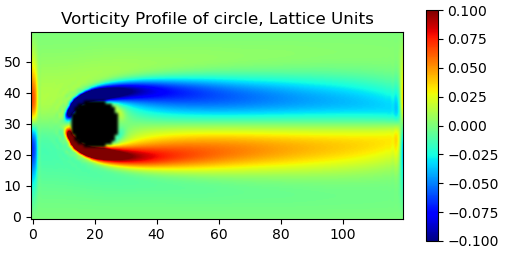
\includegraphics[width=0.65\textwidth]{final_circle.png}
\captionsetup{format = hang, width = 0.8\textwidth}
\caption{Steady-state vorticity of a circle in a 2-D wind tunnel.}
\label{fig:FinalCircle}
\end{figure}
\end{centering}

\begin{centering}
\begin{figure}[H]
\centering
\graphicspath{ {stream_images/} }
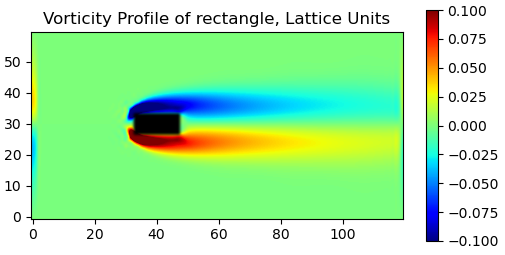
\includegraphics[width=0.65\textwidth]{final_rectangle.png}
\captionsetup{format = hang, width = 0.8\textwidth}
\caption{Steady-state vorticity of a rectangle in a 2-D wind tunnel.}
\label{fig:FinalRectangle}
\end{figure}
\end{centering}

\begin{centering}
\begin{figure}[H]
\centering
\graphicspath{ {stream_images/} }
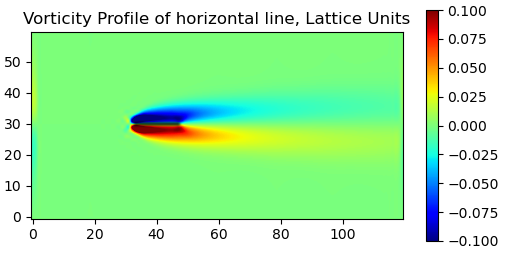
\includegraphics[width=0.65\textwidth]{final_horizontal.png}
\captionsetup{format = hang, width = 0.8\textwidth}
\caption{Steady-state vorticity of a horizontal line in a 2-D wind tunnel.}
\label{fig:FinalHorizontal}
\end{figure}
\end{centering}

\begin{centering}
\begin{figure}[H]
\centering
\graphicspath{ {stream_images/} }
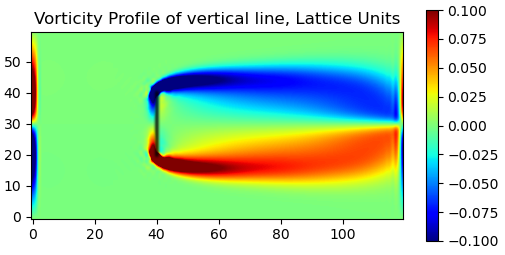
\includegraphics[width=0.65\textwidth]{final_vertical.png}
\captionsetup{format = hang, width = 0.8\textwidth}
\caption{Steady-state vorticity of a vertical line in a 2-D wind tunnel.}
\label{fig:FinalVertical}
\end{figure}
\end{centering}

\begin{centering}
\begin{figure}[H]
\centering
\graphicspath{ {stream_images/} }
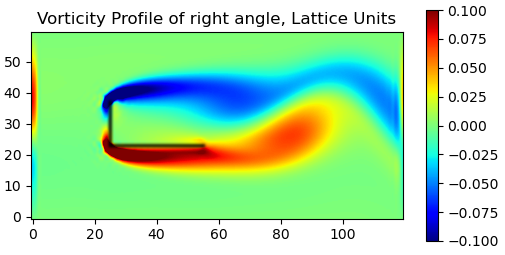
\includegraphics[width=0.65\textwidth]{final_right_angle.png}
\captionsetup{format = hang, width = 0.8\textwidth}
\caption{Steady-state vorticity of a right-angle line in a 2-D wind tunnel.}
\label{fig:FinalRightAngle}
\end{figure}
\end{centering}

\hfill


\subsection{Airfoil Wings and Stability}
\subsubsection{Stable Flow}

\begin{centering}
\begin{figure}[H]
\centering
\graphicspath{ {stream_images/} }
\subcaptionbox{\(t \approx 0\) }{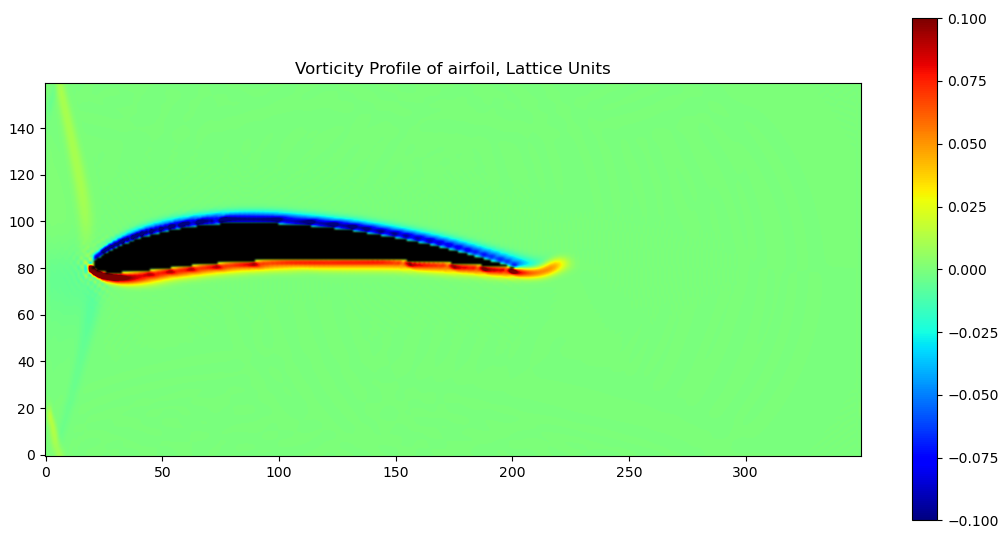
\includegraphics[width = 0.32\textwidth]{stable_airfoil_1.png}}
\hfill
\subcaptionbox{\(t > 0\)}{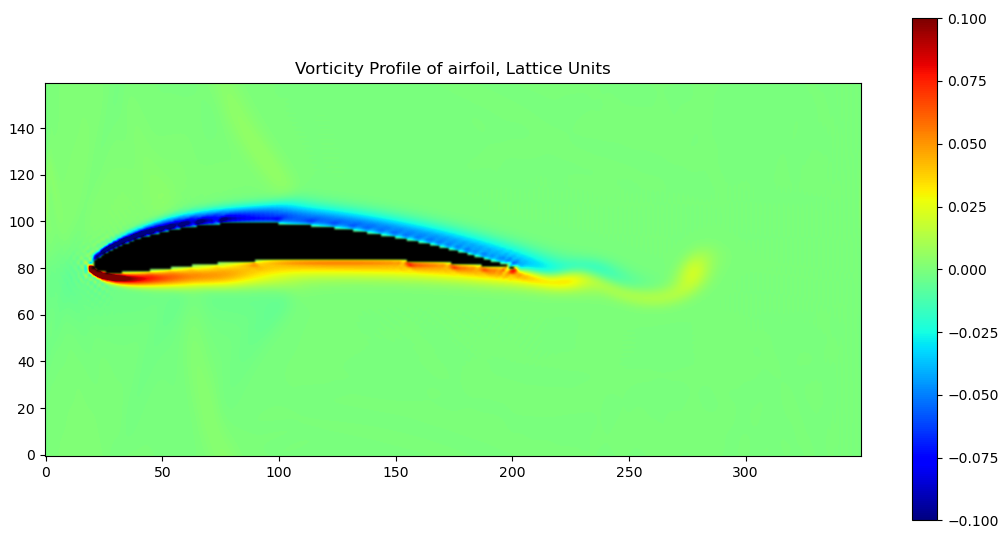
\includegraphics[width = 0.32\textwidth]{stable_airfoil_2.png}}
\hfill
\subcaptionbox{\(t >> 0\)}{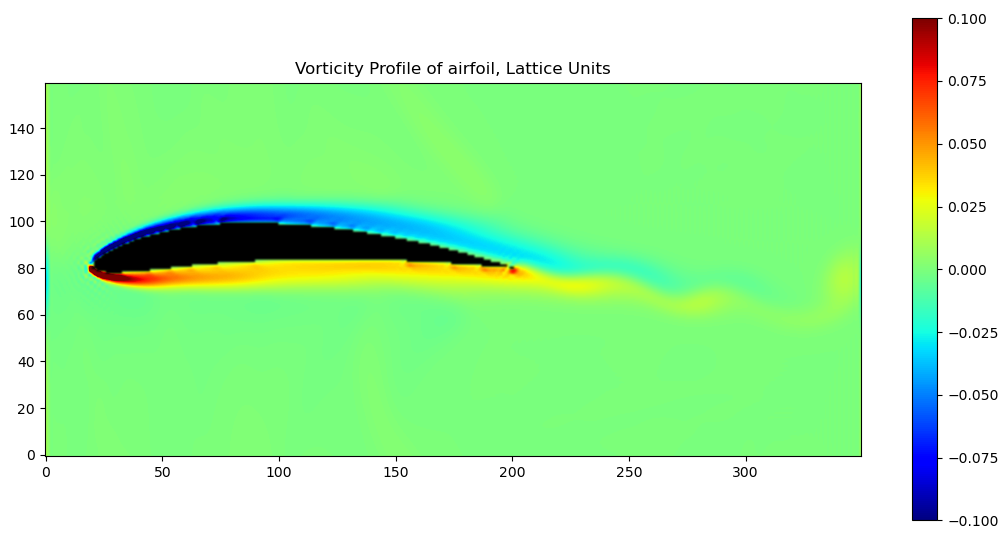
\includegraphics[width = 0.32\textwidth]{stable_airfoil_3.png}}
\label{figs:StableAirfoil}
\captionsetup{format = hang, width = 0.8\textwidth}
\caption{Time evolved vorticies of a NASA 4812 airfoil in a stable fluid flow (low velocity, high viscosity).}
\end{figure}
\end{centering}

\subsubsection{Unstable Flow}

\begin{centering}
\begin{figure}[H]
\centering
\graphicspath{ {stream_images/} }
\subcaptionbox{\(t \approx 0\) }{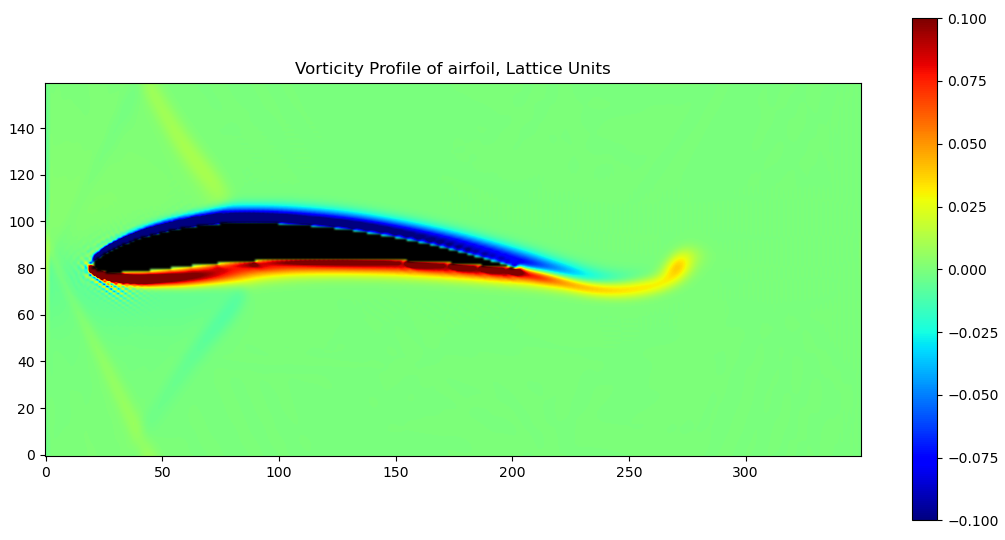
\includegraphics[width = 0.32\textwidth]{unstable_airfoil_1.png}}
\hfill
\subcaptionbox{\(t > 0\)}{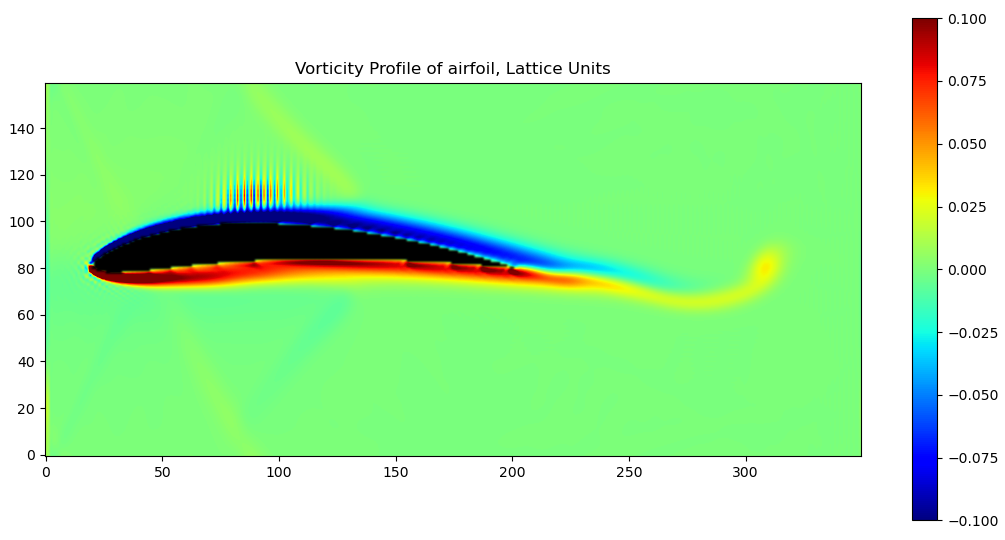
\includegraphics[width = 0.32\textwidth]{unstable_airfoil_2.png}}
\hfill
\subcaptionbox{\(t >> 0\)}{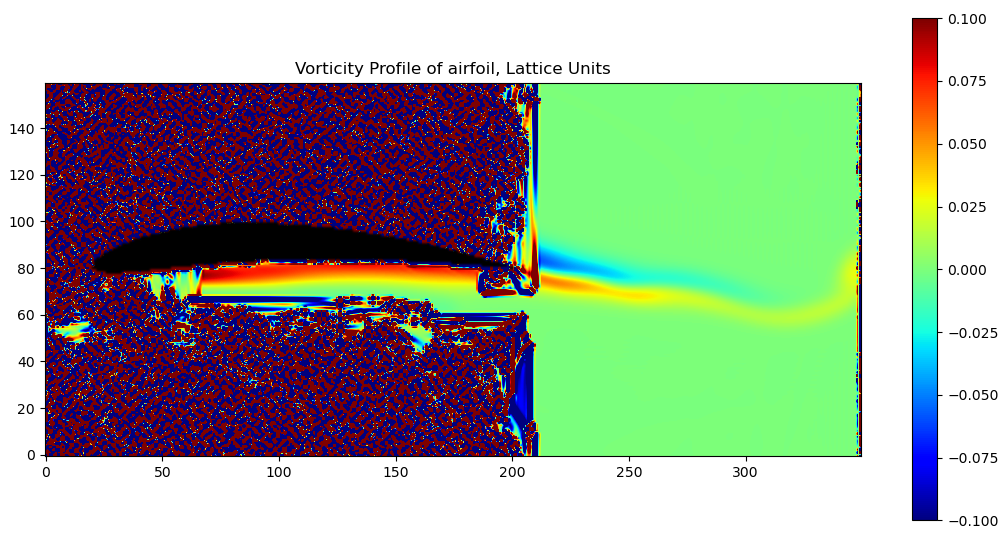
\includegraphics[width = 0.32\textwidth]{unstable_airfoil_3.png}}
\label{figs:UnstableAirfoil}
\captionsetup{format = hang, width = 0.8\textwidth}
\caption{Time evolved vortices of a NASA 4812 airfoil in an unstable fluid flow (high velocity, low viscosity). Notice the significant diversion beginning at the front of the wing.}
\end{figure}
\end{centering}






%----------------------------------------------------------------------------------------
%	REFERENCE LIST
%----------------------------------------------------------------------------------------
\newpage
\bibliography{article_2}
\bibliographystyle{ieeetr}



%----------------------------------------------------------------------------------------

\end{document}




% \noindent While LBM implementations exist in many languages (most notably C/C++ and Fortran, because of their compiled efficiency), the intent of this project is to develop an LBM framework for modeling 2-dimensional fluid flow in Julia, distributed among the  128 NVIDIA CUDA cores on the NVIDIA Jetson Nano (a development kit, much like the Raspberry Pi, optimized for things like parallel computing and AI tech). It boasts 0.5 TFLOPs, which will enable super-fast calculations for LBM, even with thousands of data points. This framework will (hopefully) be developed in such a way to also extend it to 3 dimensions in the future. Initial tests will involve creating a "wind tunnel" into which any type of shape can be placed. A simple graphical interface will be developed for ease of use, which will include sliders for viscosity, initial speed, and other necessary parameters, and will display quantities such as fluid curl, speed, and pressure. While there will be pre-defined shapes (like circles, steps, lines), the code will be modified to allow custom shapes defined by the user.\\
%
%
% \noindent Additional intentions include: modeling Poiseuille-Couette flow, modeling a water drop's evolving shape upon hitting a surface, and (potentially) adding temperature-dependent boundary conditions, which will allow a combination of heat-dependent pressures and densities (hence affecting speed). This would be an extremely interesting addition, as it would allow simple modeling of a heated aircraft wing in a very cold environment.


% Footnote example:
%Text requiring further explanation\footnote{Example footnote}.
